\documentclass{acm_proc_article-sp}
\usepackage{float}
\begin{document}

\title{Essence of Context-Oriented Programming}

\author{
\alignauthor
Ivo Willemsen\\
       \affaddr{Open Universiteit}\\
       \affaddr{Maastricht, The Netherlands}\\
       \email{ivo.willemsen@outlook.com}
}

\maketitle
\begin{abstract}
The last decade, use-cases have emerged that emphasis the need to cater for different behavior depending on situation and context changes. Examples are: Pervasive systems \cite{pervasivecomputing} and highly personalized business applications. Conventional programming languages offer constructs to implement context-dependent behavior, like  conditional branches using if/switch statements, but they often result in cluttered code and uses of those 
constructs seriously damage the modularity of the applications. In the early 2000s, a new programming paradigm emerged, called Context-Oriented Programming which targeted to mitigate the aforementioned problems by incorporating context as as part of the programming language, like variables, classes, and functions constitute the constructs 
of many contemporary languages.

This paper presents an introduction to Context-Oriented Programming, focusing on what Context-Oriented Programming is and explaining the \textit{raison d'etre} of its usage. As additional reading, examples of Context-Oriented Programming languages are given and some other aspects of these languages are elaborated on.  
\end{abstract}

\keywords{Context-Oriented Programming, context-aware systems, behavioral variations, layer activations, partial method definitions, ContextJ} 

\section{Introduction} \label{introduction}
Many applications present behavior that is determined by the context in which it is being used. Examples of different contexts are: Battery level, GPS-location, available connectivity protocols (Wifi/3G/4G), speed of the network, user's preferences, etcetera.

For example, battery level of a tablet or a smart phone on which an application (Operating System in this case) runs is a context, which probably impacts many behavioral aspects of that applications. It will not only have affect on the brightness of the screen, but it might also influence the way the Operating System prioritizes running threads, and perhaps result in the preventive hibernation of the system.

In order to include context-dependent behavior in applications using most modern programming languages, one option available is to use the Strategy Design Pattern \cite{strategypattern} to abstract the context-dependent behavior into separate classes and decide at runtime-level which context-dependent behavior (strategy) to use. Even worse would be the usage of conditional statements to find out the context in which a certain program is running, and as a result, not adhering to one of the concepts of Object-Oriented Programming: To avoid conditional statements to determine polymorphic behavior. Both options are suboptimal as they result in cluttered code which is difficult to reuse and to understand and makes maintenance of the code a very cumbersome activity.

So, behavioral variation is not implemented by a sole object, rather it is spread over a group of cooperating objects. It is called a crosscutting concern \cite{kiczalesetallaop} and this is a functionality that is dispersed over several cooperating objects. Plain old Object-Oriented Programming languages don't have constructs that allow for modularization and composition of crosscutting concerns, they lack first-class constructs. A first-class construct \cite{Keays:2003:CP:940923.940926} is a construct which is an element of a language, like a class or a method in Java. The lack of first-class constructs in regular Object-Oriented Programming languages to support the development of context-aware applications, leaves the developer of those applications with the need to implement necessary \textit{boiler-plate code}. What is needed, is a type of language that incorporates those constructs; which allow a developer to focus more on the implementation of business use-cases and less on inventing the wheel of "context determination, modularization and activation" over and over again. 

Paragraph \ref{sec:context} will zoom into the concept of "Context", which contains basic Context-Oriented Programming jargon, which will be referred to in subsequent paragraphs. Behavioral variations is introduced in paragraph \ref{sec:behavioral_variations}, whilst paragraph \ref{sec:layers} explains how to define behavioral variations in a class by using partial method definitions. Paragraph \ref{sec:layer_activation} lists the types of activations that exist in order to activate behavioral variations. 

\section{Context-Oriented Programming}
\label{cop}
In the early 2000s, a new programming paradigm appeared which is called COP (Context-Oriented Programming). This development was triggered by the appearance of a wide range of scenarios where applications had to react differently according to the active context. Conventional Object-Oriented Programming languages did not exhibit language structures that enabled developers to implement behavioral variations to changes in contexts in a modular way. 
\pagebreak
Context-Oriented Programming promotes the modularization of context-dependent behavioral variations. It offers exclusive abstractions and mechanisms in the form of first-class constructs which enables developers to effectively define entities that need to change behavior depending on their context. It allows applications to be partitioned into behavioral variations that can be activated at runtime level with predefined scopes. These behavioral variations are composed of \textit{partial definitions} for entities, like classes, functions, methods, procedures, etcetera. Context-oriented Programming offer the following functionalities whose mechanisms are implemented as part of the language \cite{Costanza:2008:CPC:1529966.1529970}:

\begin{itemize}
\item {Context}
\item Behavioral variations
\item Layers
\item Layer activation
\item Scoping
\end{itemize}

\subsection{Context}
\label{sec:context}
Context can be defined as any information that can be used to characterize the situation of an entity. An entity is a person, place or object that is considered relevant to the interaction between a user and an application, including the user and the application themselves \cite{Abowd:1999:TBU:647985.743843}. Context is derived from three sources: Environment, system and the actors. Contextual information that originates from actors and the environment is information that reaches the system from outside, but the system itself can also generate context. 

A \textit{system} is a set of computational objects, methods, functions that responds with predefined behavior on per-request basis. An \textit{actor} is a person or another system that is directly involved with the system: It determines the order in which use-cases are executed by communicating directly with the system, by clicking on buttons, sending messages, receiving feedback, etcetera. An example of context generated by an actor is the differences in behavior that originate from the choices made by a user when accessing certain functionalities. Another example is the support of multiple devices (like an smart phone or a desktop computer) that add to the context-dependent behavior of the system. The \textit{environment} encompasses everything that lies outside the boundaries of the system, and which is not directly involved in the relationship between the system and the actors.

behavioral variations, changes in response, depend on the context that is generated by these three sources. As a result, context-dependent behavior variations can be split up into actor-dependent, environmental- dependent and system-dependent variations.

\textit{Context} is information that can be computationally accessed in a software system. This definition is kind of vague, as it leaves room for a variety of interpretations: 
\begin{itemize}
\item The definition does not specify whether the information should originate from outside of the system, the environment, but is also comes from other sources like the actors and the system itself.
\item The granularity of abstraction is not enforced by the definition. Context can exist in the system, or can come to the system as fine-grained pieces of information, like in-discrete numerical temperature indications and can subsequently be transformed to more course-grained information classes like "low", "medium", "high". 
\item The uniqueness of the context is not imposed. There exist implementations of Context-Oriented Programming languages that enable applications to share only a common context. Other implementations don't follow this model and allow several contexts to exist, which are used in different parts of the application \cite{Appeltauer:2009:CCP:1562112.1562118}
\end{itemize}

\subsection{Behavioral variations}
\label{sec:behavioral_variations}
Context-Oriented Programming languages have first-class constructs that support \textit{behavioral variations} by means of partial definition of modules. behavioral variations can be expressed in terms of new behavior, modified behavior or behavior that has been removed. The first-class constructs that are involved in these concepts are plain Object-oriented Programming constructs like classes and methods. behavioral variations can be \textit{activated}, partly changing the behavior of the application. So, the function of behavior variations is to allow \textit{runtime activation} of a change in behavior, and it also allows for the \textit{modularization} of behavior by exploiting the available constructs in the Context-Oriented Programming language.    

\subsection{Layers}
\label{sec:layers}
\textit{Layers} group contextual-dependent behavioral variations as first-class entities that can be explicitly referred to in a program at runtime. Layers are first-class entities in most Context-Oriented Programming languages, which groups partial definitions and can be stored in variables and passed to methods. Several parts of the application can have access to the same layers and determine the exact changes in behavior that have to be done. In case of layers, the first-class entity that implements this functionality is a layered method. This method consists of a base, principle method definition, extended with at least one extra partial definition. The root layer that is always present, that represents the base definition, defines the context-independent behavior of the application.

\begin{figure}[H]
\centering
\fbox{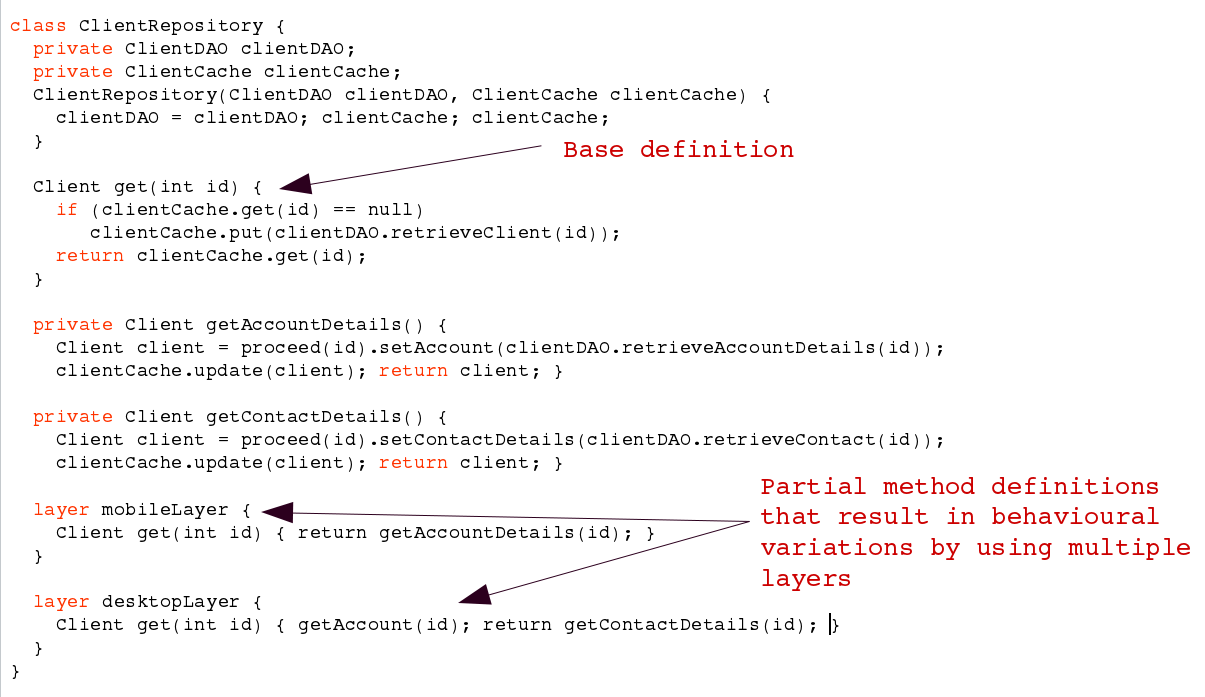
\includegraphics[width=70mm]{layers.png}}
\caption{Layers, behavioral variations and base/partial definition}
\label{fig:layers}
\end{figure}

The code snippets like the above and in other figures in this paper, are based on the ContextJ implementation (Java-based) \cite{Appeltauer:2009:IDC:1562112.1562117}, but are by no means meant to be compile-ready as they only serve an explanatory goal. In the above figure, the base behavior of the ClientRepository is to only retrieve the client information. The base definition of the get-method first checks the cache for the presence of the object that is associated with the id that is passed in. If found, it returns that object, if not found, it will get the object from the underlying data store, through the DAO-object (\textit{Data Access Object}). 

The get-method is partially redefined in two layers that are defined in the same class by making use of the first-class construct "layer". In case the account layer is active, first the base functionality of the get-method will be invoked by the proceed-call. After the proceed-call has retrieved the object, the partial definition will make a call to the DAO object in order to retrieve the account information that is related with the client. Before returning the object to the caller, the partial definition will make sure that the cache is updated with the newly retrieved information. 

So, based on the use-case, account and/or contact information can be \textit{lazily loaded}, by activating the corresponding layers, achieving a simple context-dependent and performance-wise efficient solution. Of course, the above use-case and sample implementation is a very simplified abstraction of what could be a real solution.

Figure \ref{fig:layers} depicts the modularization and definition of the behavioral variations by using layers. The next paragraph focuses on the activation of the layers.

\subsection{Layer activation}
\label{sec:layer_activation}
\textit{Layer activation} is achieved by language constructs that ensure that layers are added at runtime, such that the certain partial method definitions have an influence on the actual behavior of an application. By default, only the root layer is active at runtime. So only the base definition associated with the root layer will directly influence the behavior of the application. Other layers 



\textit{Scoping} of layer activation and deactivation ensures that
the behavioral variations are only effective for welldefined
parts of a program, and for well-defined durations.

ref no 6.!!!1 relationship between activation and beh var.

\bibliographystyle{abbrv}
\bibliography{sigproc}
\end{document}
